% Options for packages loaded elsewhere
\PassOptionsToPackage{unicode}{hyperref}
\PassOptionsToPackage{hyphens}{url}
\PassOptionsToPackage{dvipsnames,svgnames,x11names}{xcolor}
%
\documentclass[
  letterpaper,
  DIV=11,
  numbers=noendperiod]{scrartcl}

\usepackage{amsmath,amssymb}
\usepackage{iftex}
\ifPDFTeX
  \usepackage[T1]{fontenc}
  \usepackage[utf8]{inputenc}
  \usepackage{textcomp} % provide euro and other symbols
\else % if luatex or xetex
  \usepackage{unicode-math}
  \defaultfontfeatures{Scale=MatchLowercase}
  \defaultfontfeatures[\rmfamily]{Ligatures=TeX,Scale=1}
\fi
\usepackage{lmodern}
\ifPDFTeX\else  
    % xetex/luatex font selection
\fi
% Use upquote if available, for straight quotes in verbatim environments
\IfFileExists{upquote.sty}{\usepackage{upquote}}{}
\IfFileExists{microtype.sty}{% use microtype if available
  \usepackage[]{microtype}
  \UseMicrotypeSet[protrusion]{basicmath} % disable protrusion for tt fonts
}{}
\makeatletter
\@ifundefined{KOMAClassName}{% if non-KOMA class
  \IfFileExists{parskip.sty}{%
    \usepackage{parskip}
  }{% else
    \setlength{\parindent}{0pt}
    \setlength{\parskip}{6pt plus 2pt minus 1pt}}
}{% if KOMA class
  \KOMAoptions{parskip=half}}
\makeatother
\usepackage{xcolor}
\setlength{\emergencystretch}{3em} % prevent overfull lines
\setcounter{secnumdepth}{-\maxdimen} % remove section numbering
% Make \paragraph and \subparagraph free-standing
\ifx\paragraph\undefined\else
  \let\oldparagraph\paragraph
  \renewcommand{\paragraph}[1]{\oldparagraph{#1}\mbox{}}
\fi
\ifx\subparagraph\undefined\else
  \let\oldsubparagraph\subparagraph
  \renewcommand{\subparagraph}[1]{\oldsubparagraph{#1}\mbox{}}
\fi

\usepackage{color}
\usepackage{fancyvrb}
\newcommand{\VerbBar}{|}
\newcommand{\VERB}{\Verb[commandchars=\\\{\}]}
\DefineVerbatimEnvironment{Highlighting}{Verbatim}{commandchars=\\\{\}}
% Add ',fontsize=\small' for more characters per line
\usepackage{framed}
\definecolor{shadecolor}{RGB}{241,243,245}
\newenvironment{Shaded}{\begin{snugshade}}{\end{snugshade}}
\newcommand{\AlertTok}[1]{\textcolor[rgb]{0.68,0.00,0.00}{#1}}
\newcommand{\AnnotationTok}[1]{\textcolor[rgb]{0.37,0.37,0.37}{#1}}
\newcommand{\AttributeTok}[1]{\textcolor[rgb]{0.40,0.45,0.13}{#1}}
\newcommand{\BaseNTok}[1]{\textcolor[rgb]{0.68,0.00,0.00}{#1}}
\newcommand{\BuiltInTok}[1]{\textcolor[rgb]{0.00,0.23,0.31}{#1}}
\newcommand{\CharTok}[1]{\textcolor[rgb]{0.13,0.47,0.30}{#1}}
\newcommand{\CommentTok}[1]{\textcolor[rgb]{0.37,0.37,0.37}{#1}}
\newcommand{\CommentVarTok}[1]{\textcolor[rgb]{0.37,0.37,0.37}{\textit{#1}}}
\newcommand{\ConstantTok}[1]{\textcolor[rgb]{0.56,0.35,0.01}{#1}}
\newcommand{\ControlFlowTok}[1]{\textcolor[rgb]{0.00,0.23,0.31}{#1}}
\newcommand{\DataTypeTok}[1]{\textcolor[rgb]{0.68,0.00,0.00}{#1}}
\newcommand{\DecValTok}[1]{\textcolor[rgb]{0.68,0.00,0.00}{#1}}
\newcommand{\DocumentationTok}[1]{\textcolor[rgb]{0.37,0.37,0.37}{\textit{#1}}}
\newcommand{\ErrorTok}[1]{\textcolor[rgb]{0.68,0.00,0.00}{#1}}
\newcommand{\ExtensionTok}[1]{\textcolor[rgb]{0.00,0.23,0.31}{#1}}
\newcommand{\FloatTok}[1]{\textcolor[rgb]{0.68,0.00,0.00}{#1}}
\newcommand{\FunctionTok}[1]{\textcolor[rgb]{0.28,0.35,0.67}{#1}}
\newcommand{\ImportTok}[1]{\textcolor[rgb]{0.00,0.46,0.62}{#1}}
\newcommand{\InformationTok}[1]{\textcolor[rgb]{0.37,0.37,0.37}{#1}}
\newcommand{\KeywordTok}[1]{\textcolor[rgb]{0.00,0.23,0.31}{#1}}
\newcommand{\NormalTok}[1]{\textcolor[rgb]{0.00,0.23,0.31}{#1}}
\newcommand{\OperatorTok}[1]{\textcolor[rgb]{0.37,0.37,0.37}{#1}}
\newcommand{\OtherTok}[1]{\textcolor[rgb]{0.00,0.23,0.31}{#1}}
\newcommand{\PreprocessorTok}[1]{\textcolor[rgb]{0.68,0.00,0.00}{#1}}
\newcommand{\RegionMarkerTok}[1]{\textcolor[rgb]{0.00,0.23,0.31}{#1}}
\newcommand{\SpecialCharTok}[1]{\textcolor[rgb]{0.37,0.37,0.37}{#1}}
\newcommand{\SpecialStringTok}[1]{\textcolor[rgb]{0.13,0.47,0.30}{#1}}
\newcommand{\StringTok}[1]{\textcolor[rgb]{0.13,0.47,0.30}{#1}}
\newcommand{\VariableTok}[1]{\textcolor[rgb]{0.07,0.07,0.07}{#1}}
\newcommand{\VerbatimStringTok}[1]{\textcolor[rgb]{0.13,0.47,0.30}{#1}}
\newcommand{\WarningTok}[1]{\textcolor[rgb]{0.37,0.37,0.37}{\textit{#1}}}

\providecommand{\tightlist}{%
  \setlength{\itemsep}{0pt}\setlength{\parskip}{0pt}}\usepackage{longtable,booktabs,array}
\usepackage{calc} % for calculating minipage widths
% Correct order of tables after \paragraph or \subparagraph
\usepackage{etoolbox}
\makeatletter
\patchcmd\longtable{\par}{\if@noskipsec\mbox{}\fi\par}{}{}
\makeatother
% Allow footnotes in longtable head/foot
\IfFileExists{footnotehyper.sty}{\usepackage{footnotehyper}}{\usepackage{footnote}}
\makesavenoteenv{longtable}
\usepackage{graphicx}
\makeatletter
\def\maxwidth{\ifdim\Gin@nat@width>\linewidth\linewidth\else\Gin@nat@width\fi}
\def\maxheight{\ifdim\Gin@nat@height>\textheight\textheight\else\Gin@nat@height\fi}
\makeatother
% Scale images if necessary, so that they will not overflow the page
% margins by default, and it is still possible to overwrite the defaults
% using explicit options in \includegraphics[width, height, ...]{}
\setkeys{Gin}{width=\maxwidth,height=\maxheight,keepaspectratio}
% Set default figure placement to htbp
\makeatletter
\def\fps@figure{htbp}
\makeatother

\KOMAoption{captions}{tableheading}
\makeatletter
\@ifpackageloaded{caption}{}{\usepackage{caption}}
\AtBeginDocument{%
\ifdefined\contentsname
  \renewcommand*\contentsname{Table of contents}
\else
  \newcommand\contentsname{Table of contents}
\fi
\ifdefined\listfigurename
  \renewcommand*\listfigurename{List of Figures}
\else
  \newcommand\listfigurename{List of Figures}
\fi
\ifdefined\listtablename
  \renewcommand*\listtablename{List of Tables}
\else
  \newcommand\listtablename{List of Tables}
\fi
\ifdefined\figurename
  \renewcommand*\figurename{Figure}
\else
  \newcommand\figurename{Figure}
\fi
\ifdefined\tablename
  \renewcommand*\tablename{Table}
\else
  \newcommand\tablename{Table}
\fi
}
\@ifpackageloaded{float}{}{\usepackage{float}}
\floatstyle{ruled}
\@ifundefined{c@chapter}{\newfloat{codelisting}{h}{lop}}{\newfloat{codelisting}{h}{lop}[chapter]}
\floatname{codelisting}{Listing}
\newcommand*\listoflistings{\listof{codelisting}{List of Listings}}
\makeatother
\makeatletter
\makeatother
\makeatletter
\@ifpackageloaded{caption}{}{\usepackage{caption}}
\@ifpackageloaded{subcaption}{}{\usepackage{subcaption}}
\makeatother
\ifLuaTeX
\usepackage[bidi=basic]{babel}
\else
\usepackage[bidi=default]{babel}
\fi
\babelprovide[main,import]{british}
% get rid of language-specific shorthands (see #6817):
\let\LanguageShortHands\languageshorthands
\def\languageshorthands#1{}
\ifLuaTeX
  \usepackage{selnolig}  % disable illegal ligatures
\fi
\usepackage{bookmark}

\IfFileExists{xurl.sty}{\usepackage{xurl}}{} % add URL line breaks if available
\urlstyle{same} % disable monospaced font for URLs
\hypersetup{
  pdftitle={Classification of Business Activities by Machine Learning: The Case of France.},
  pdfauthor={Nathan Randriamanana},
  pdflang={en-GB},
  colorlinks=true,
  linkcolor={blue},
  filecolor={Maroon},
  citecolor={Blue},
  urlcolor={Blue},
  pdfcreator={LaTeX via pandoc}}

\title{Classification of Business Activities by Machine Learning: The
Case of France.}
\author{\href{https://github.com/TheAIWizard}{Nathan Randriamanana}}
\date{30 April 2024}

\begin{document}
\maketitle

\subsection{Context}\label{context}

\begin{itemize}
\tightlist
\item
  {\textbf{Sirene}} is the French national company registry
\item
  When a company registers, an {\textbf{activity code}} is attributed
\item
  Early 2023: Sirene 3 -\textgreater{} Sirene 4:

  \begin{itemize}
  \tightlist
  \item
    Refactoring of the Sirene {\textbf{information system}} :
  \item
    Companies register through a {\textbf{new channel}}
  \item
    {\textbf{Performance drop}} of the legacy coding engine
  \item
    Teams already {\textbf{overwhelmed}}
  \end{itemize}
\item
  {\textbf{Consequence}}: Ideal moment to innovate (but under the
  constraint!)
\end{itemize}

\subsection{The administrative ``flow'' of
formalities}\label{the-administrative-flow-of-formalities}

\begin{itemize}
\tightlist
\item
  Siren number: company directory identification system
\item
  Classification on a daily basis
\item
  Different administrations ==\textgreater{} information systems
  ==\textgreater{} Need to be quick, responsive and flexible to updated
  instructions
\end{itemize}

registrant -\textgreater{} GUE -\textgreater{} XML -\textgreater{}

\begin{center}
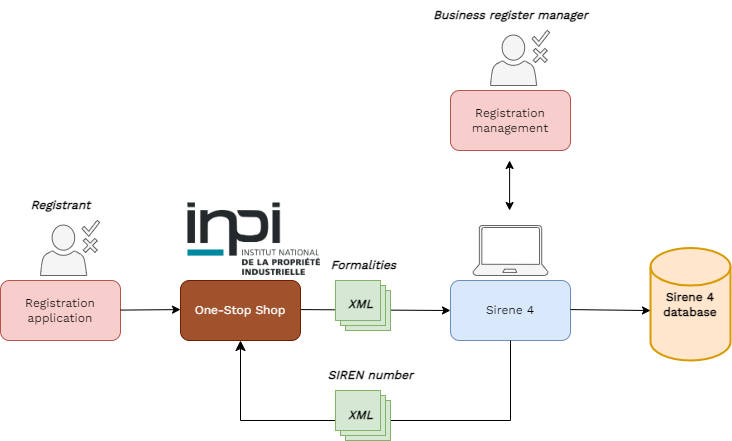
\includegraphics{../img/flow-formalities.png}
\end{center}

\subsection{Assign an activy code: 2
ways}\label{assign-an-activy-code-2-ways}

\begin{center}
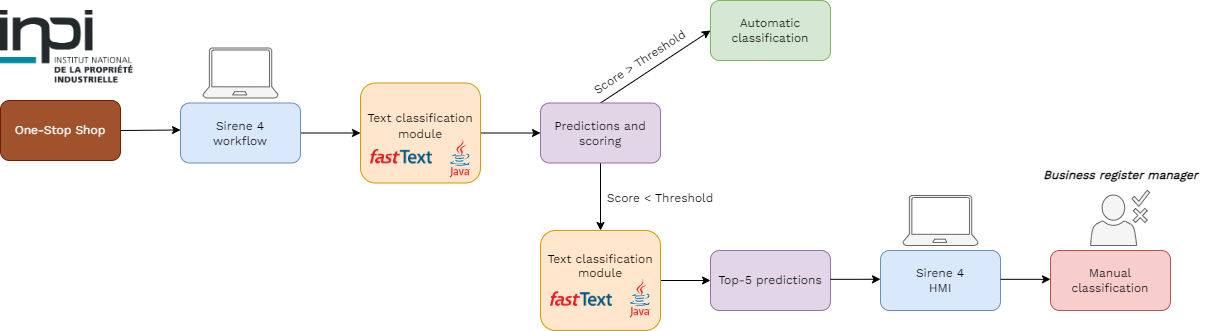
\includegraphics{../img/orga-post-prod-sirene4-en.png}
\end{center}

\subsection{Near-ubiquity of ML}\label{near-ubiquity-of-ml}

\begin{center}
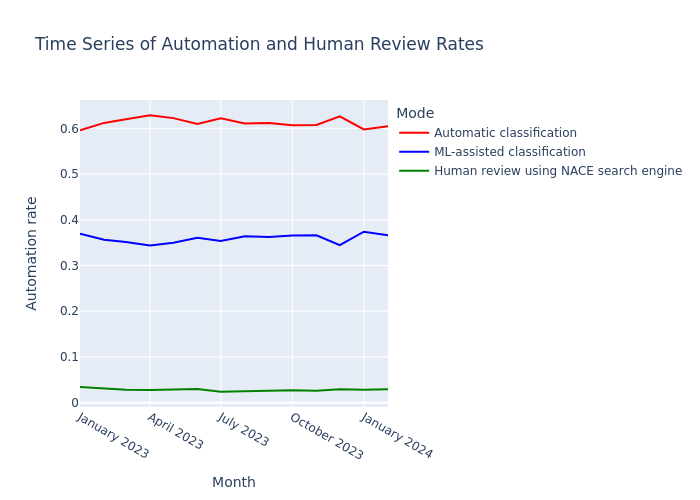
\includegraphics{../img/automation_rate.png}
\end{center}

\subsection{Human review}\label{human-review}

\begin{center}
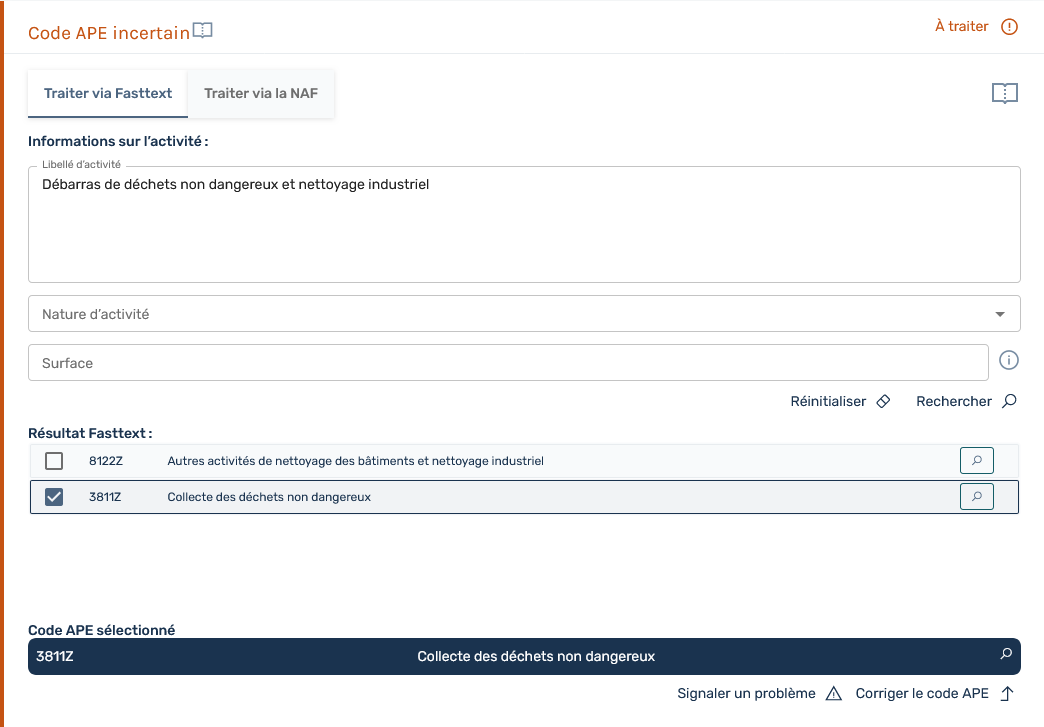
\includegraphics{../img/reprise_gestionnaire_ape.png}
\end{center}

\subsection{Human review}\label{human-review-1}

\begin{center}
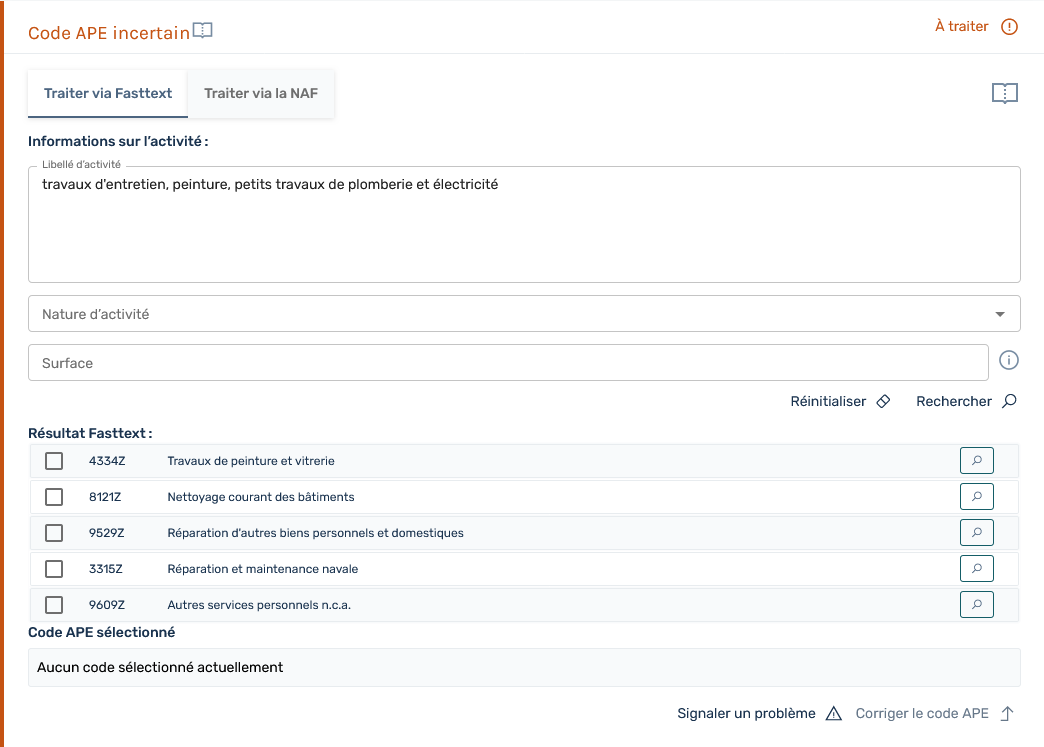
\includegraphics{../img/reprise_gestionnaire_manque_contexte.png}
\end{center}

\subsection{Model}\label{model}

\begin{itemize}
\tightlist
\item
  {\textbf{Text classification}} model which uses additional categorical
  variables
\item
  For now we use the {\textbf{fastText}} library
\item
  Originally trained on legacy data annotated partly by the
  {\textbf{coding engine}} and partly {\textbf{manually}}
\end{itemize}

\subsection{FastText}\label{fasttext}

\begin{center}
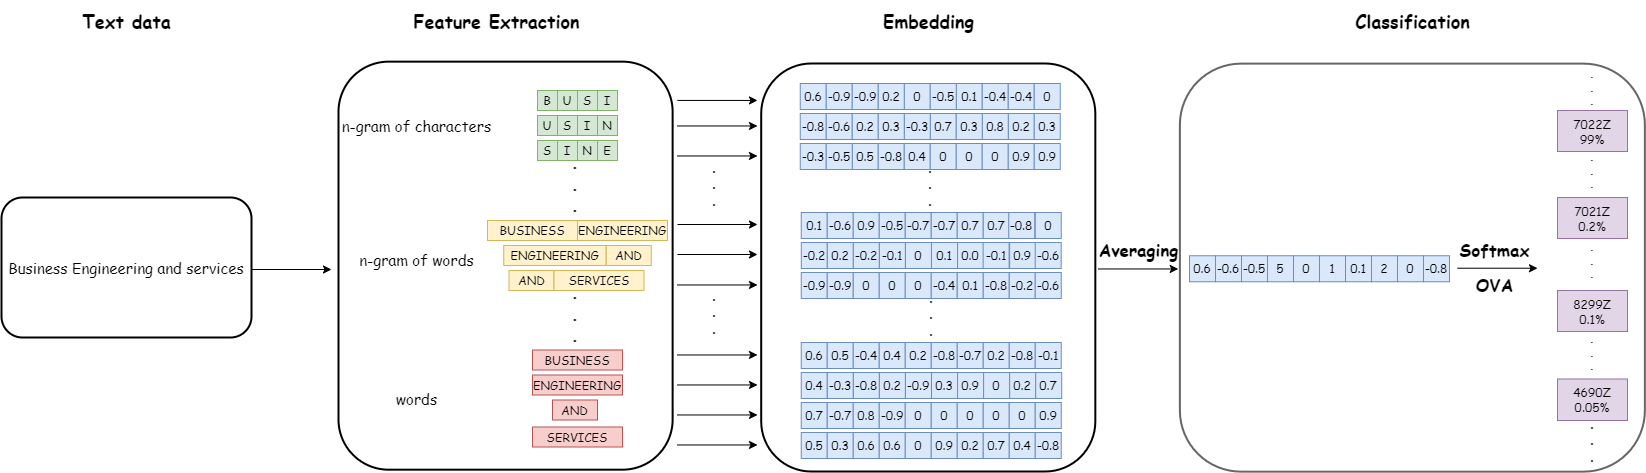
\includegraphics{../img/diag-fasttext-rectif.pdf}
\end{center}

\subsection{FastText}\label{fasttext-1}

\begin{center}
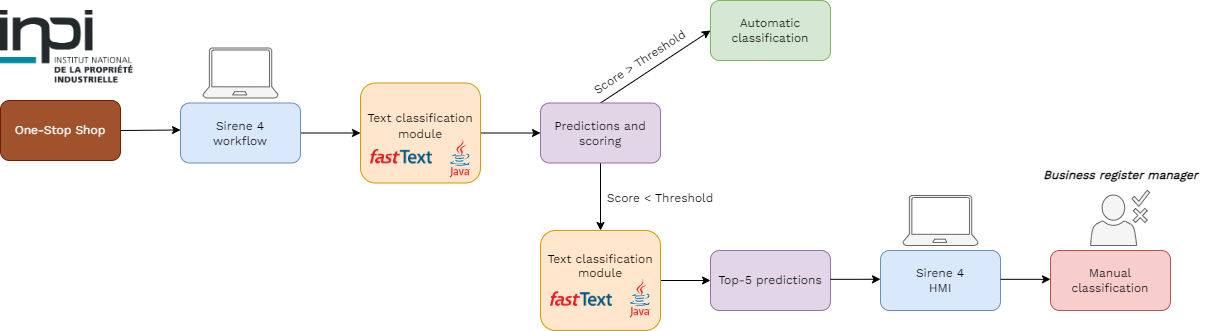
\includegraphics{../img/orga-post-prod-sirene4-en.png}
\end{center}

\subsection{Current state of affairs}\label{current-state-of-affairs}

\begin{itemize}
\tightlist
\item
  Model trained on Insee's {\textbf{cloud data science platform}} 😍
\item
  Coding engine {\textbf{developed in Java}} inside of a monolithic
  architecture 😫

  \begin{itemize}
  \tightlist
  \item
    {\textbf{Code duplication}}
  \item
    {\textbf{Reproductibility}} issues
  \item
    {\textbf{Increased risk}} of error
  \item
    {\textbf{Maintenance problems}}
  \item
    {\textbf{No monitoring}}
  \item
    {\textbf{No test data}}
  \end{itemize}
\end{itemize}

\subsection{Current state of affairs}\label{current-state-of-affairs-1}

\begin{center}
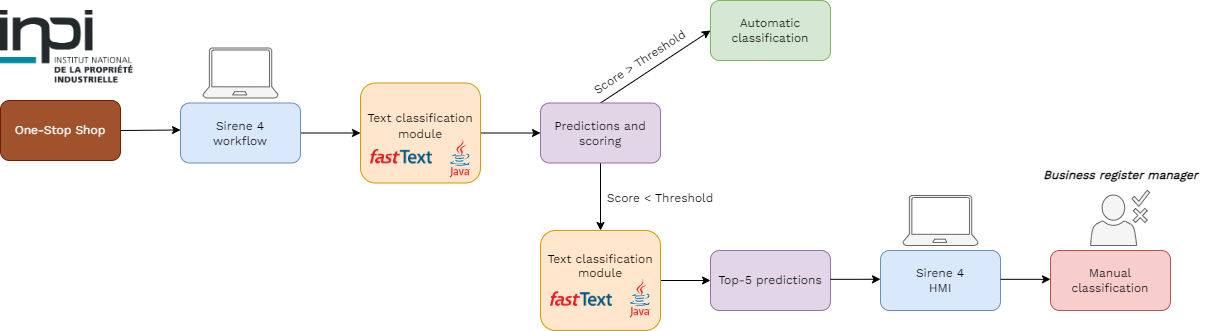
\includegraphics{../img/orga-post-prod-sirene4-en.png}
\end{center}

\subsection{MLOps target}\label{mlops-target}

\begin{itemize}
\tightlist
\item
  Microservice architecture running on a {\textbf{Kubernetes cluster}}

  \begin{itemize}
  \tightlist
  \item
    Experiment tracking and model store: {\textbf{MLflow}}
  \item
    Model served via an API: {\textbf{FastAPI}}
  \item
    Automation with {\textbf{ArgoCD}}
  \item
    Monitoring dashboard: {\textbf{Quarto}} and {\textbf{DuckDB}}
  \item
    Quality control: annotations with {\textbf{Label Studio}}
  \end{itemize}
\end{itemize}

\subsection{Experiment tracking}\label{experiment-tracking}

\begin{itemize}
\tightlist
\item
  {\textbf{Argo Workflows}} used for \emph{distributed} training
\item
  {\textbf{MLflow}} used to track/log experiments and compare runs
\end{itemize}

\subsection{Model store}\label{model-store}

\begin{itemize}
\tightlist
\item
  {\textbf{MLflow}} also used as a model store
\item
  Models are packaged with all the metadata necessary to {\textbf{run
  inference}}
\item
  Registered models are {\textbf{simply loaded}} with this command where
  \texttt{version} is a number or a \texttt{"Production"} tag for
  example
\end{itemize}

\begin{Shaded}
\begin{Highlighting}[]
\NormalTok{model }\OperatorTok{=}\NormalTok{ mlflow.pyfunc.load\_model(}
\NormalTok{    model\_uri}\OperatorTok{=}\SpecialStringTok{f"models:/}\SpecialCharTok{\{}\NormalTok{model\_name}\SpecialCharTok{\}}\SpecialStringTok{/}\SpecialCharTok{\{}\NormalTok{version}\SpecialCharTok{\}}\SpecialStringTok{"}
\NormalTok{)}
\end{Highlighting}
\end{Shaded}

\subsection{API serving}\label{api-serving}

\begin{itemize}
\tightlist
\item
  Text classification model served through a containerized {\textbf{REST
  API}}:

  \begin{itemize}
  \tightlist
  \item
    {\textbf{Simplicity}} for end users
  \item
    {\textbf{Standard query format}}
  \item
    {\textbf{Scalable}}
  \item
    {\textbf{Modular}} and {\textbf{portable}}
  \end{itemize}
\item
  {\textbf{Multiple endpoints}}: batch, online
\item
  Continuous deployment with {\textbf{Argo CD}}
\end{itemize}

\subsection{API serving}\label{api-serving-1}

\begin{center}
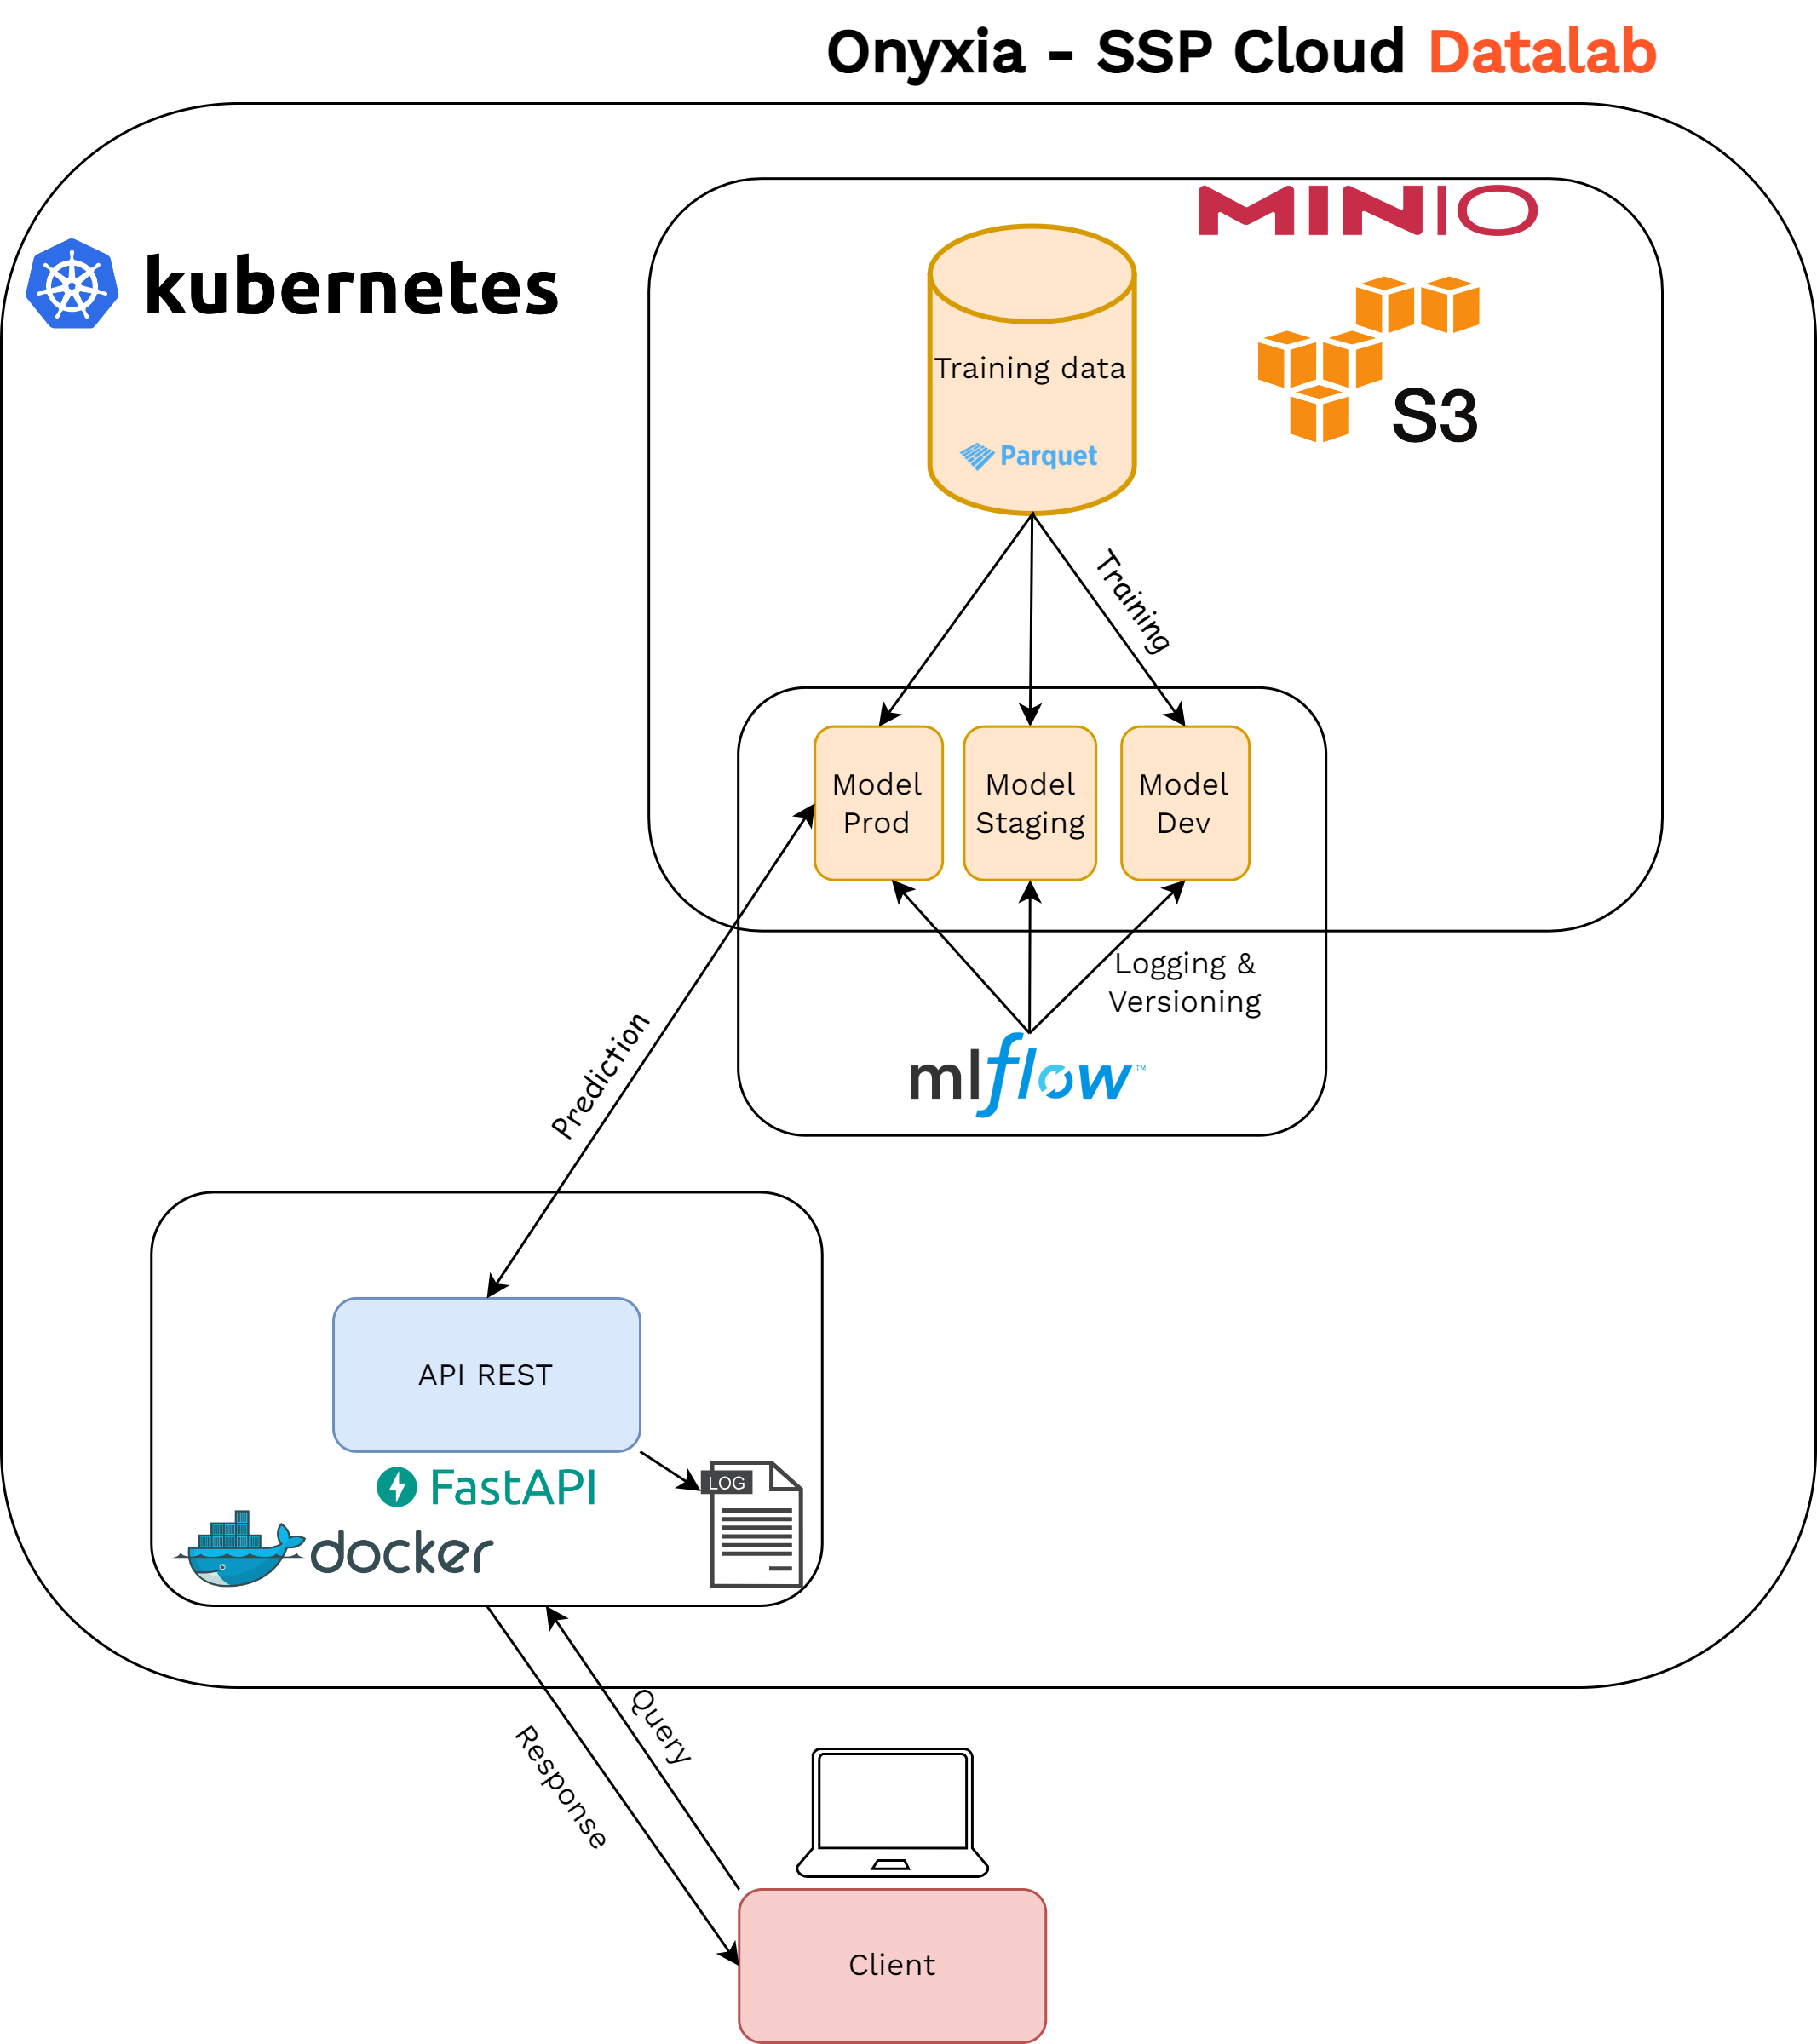
\includegraphics{../img/api-datalab.png}
\end{center}

\subsection{Monitoring}\label{monitoring}

\begin{itemize}
\tightlist
\item
  {\textbf{Monitoring}} the model in a production environment is
  necessary:

  \begin{itemize}
  \tightlist
  \item
    To detect {\textbf{distribution drifts}} in input data
  \item
    To check that the model has a {\textbf{stable behavior}}
  \item
    To decide {\textbf{when to retrain}} a model
  \end{itemize}
\item
  Ideally, we would like to track model {\textbf{accuracy in real-time}}
  but expensive
\item
  In addition, monitoring of the API: {\textbf{latency}},
  {\textbf{memory managment}}, {\textbf{disk usage}}, etc.
\end{itemize}

\subsection{Monitoring}\label{monitoring-1}

\begin{itemize}
\tightlist
\item
  {\textbf{How}} we do it:

  \begin{itemize}
  \tightlist
  \item
    API {\textbf{logs}} its activity
  \item
    Logs are fetched and formatted {\textbf{periodically}}
  \item
    {\textbf{Metrics}} are computed from the formatted logs
  \item
    Display on a {\textbf{dashboard}}
  \end{itemize}
\end{itemize}

\subsection{Monitoring}\label{monitoring-2}

\begin{center}
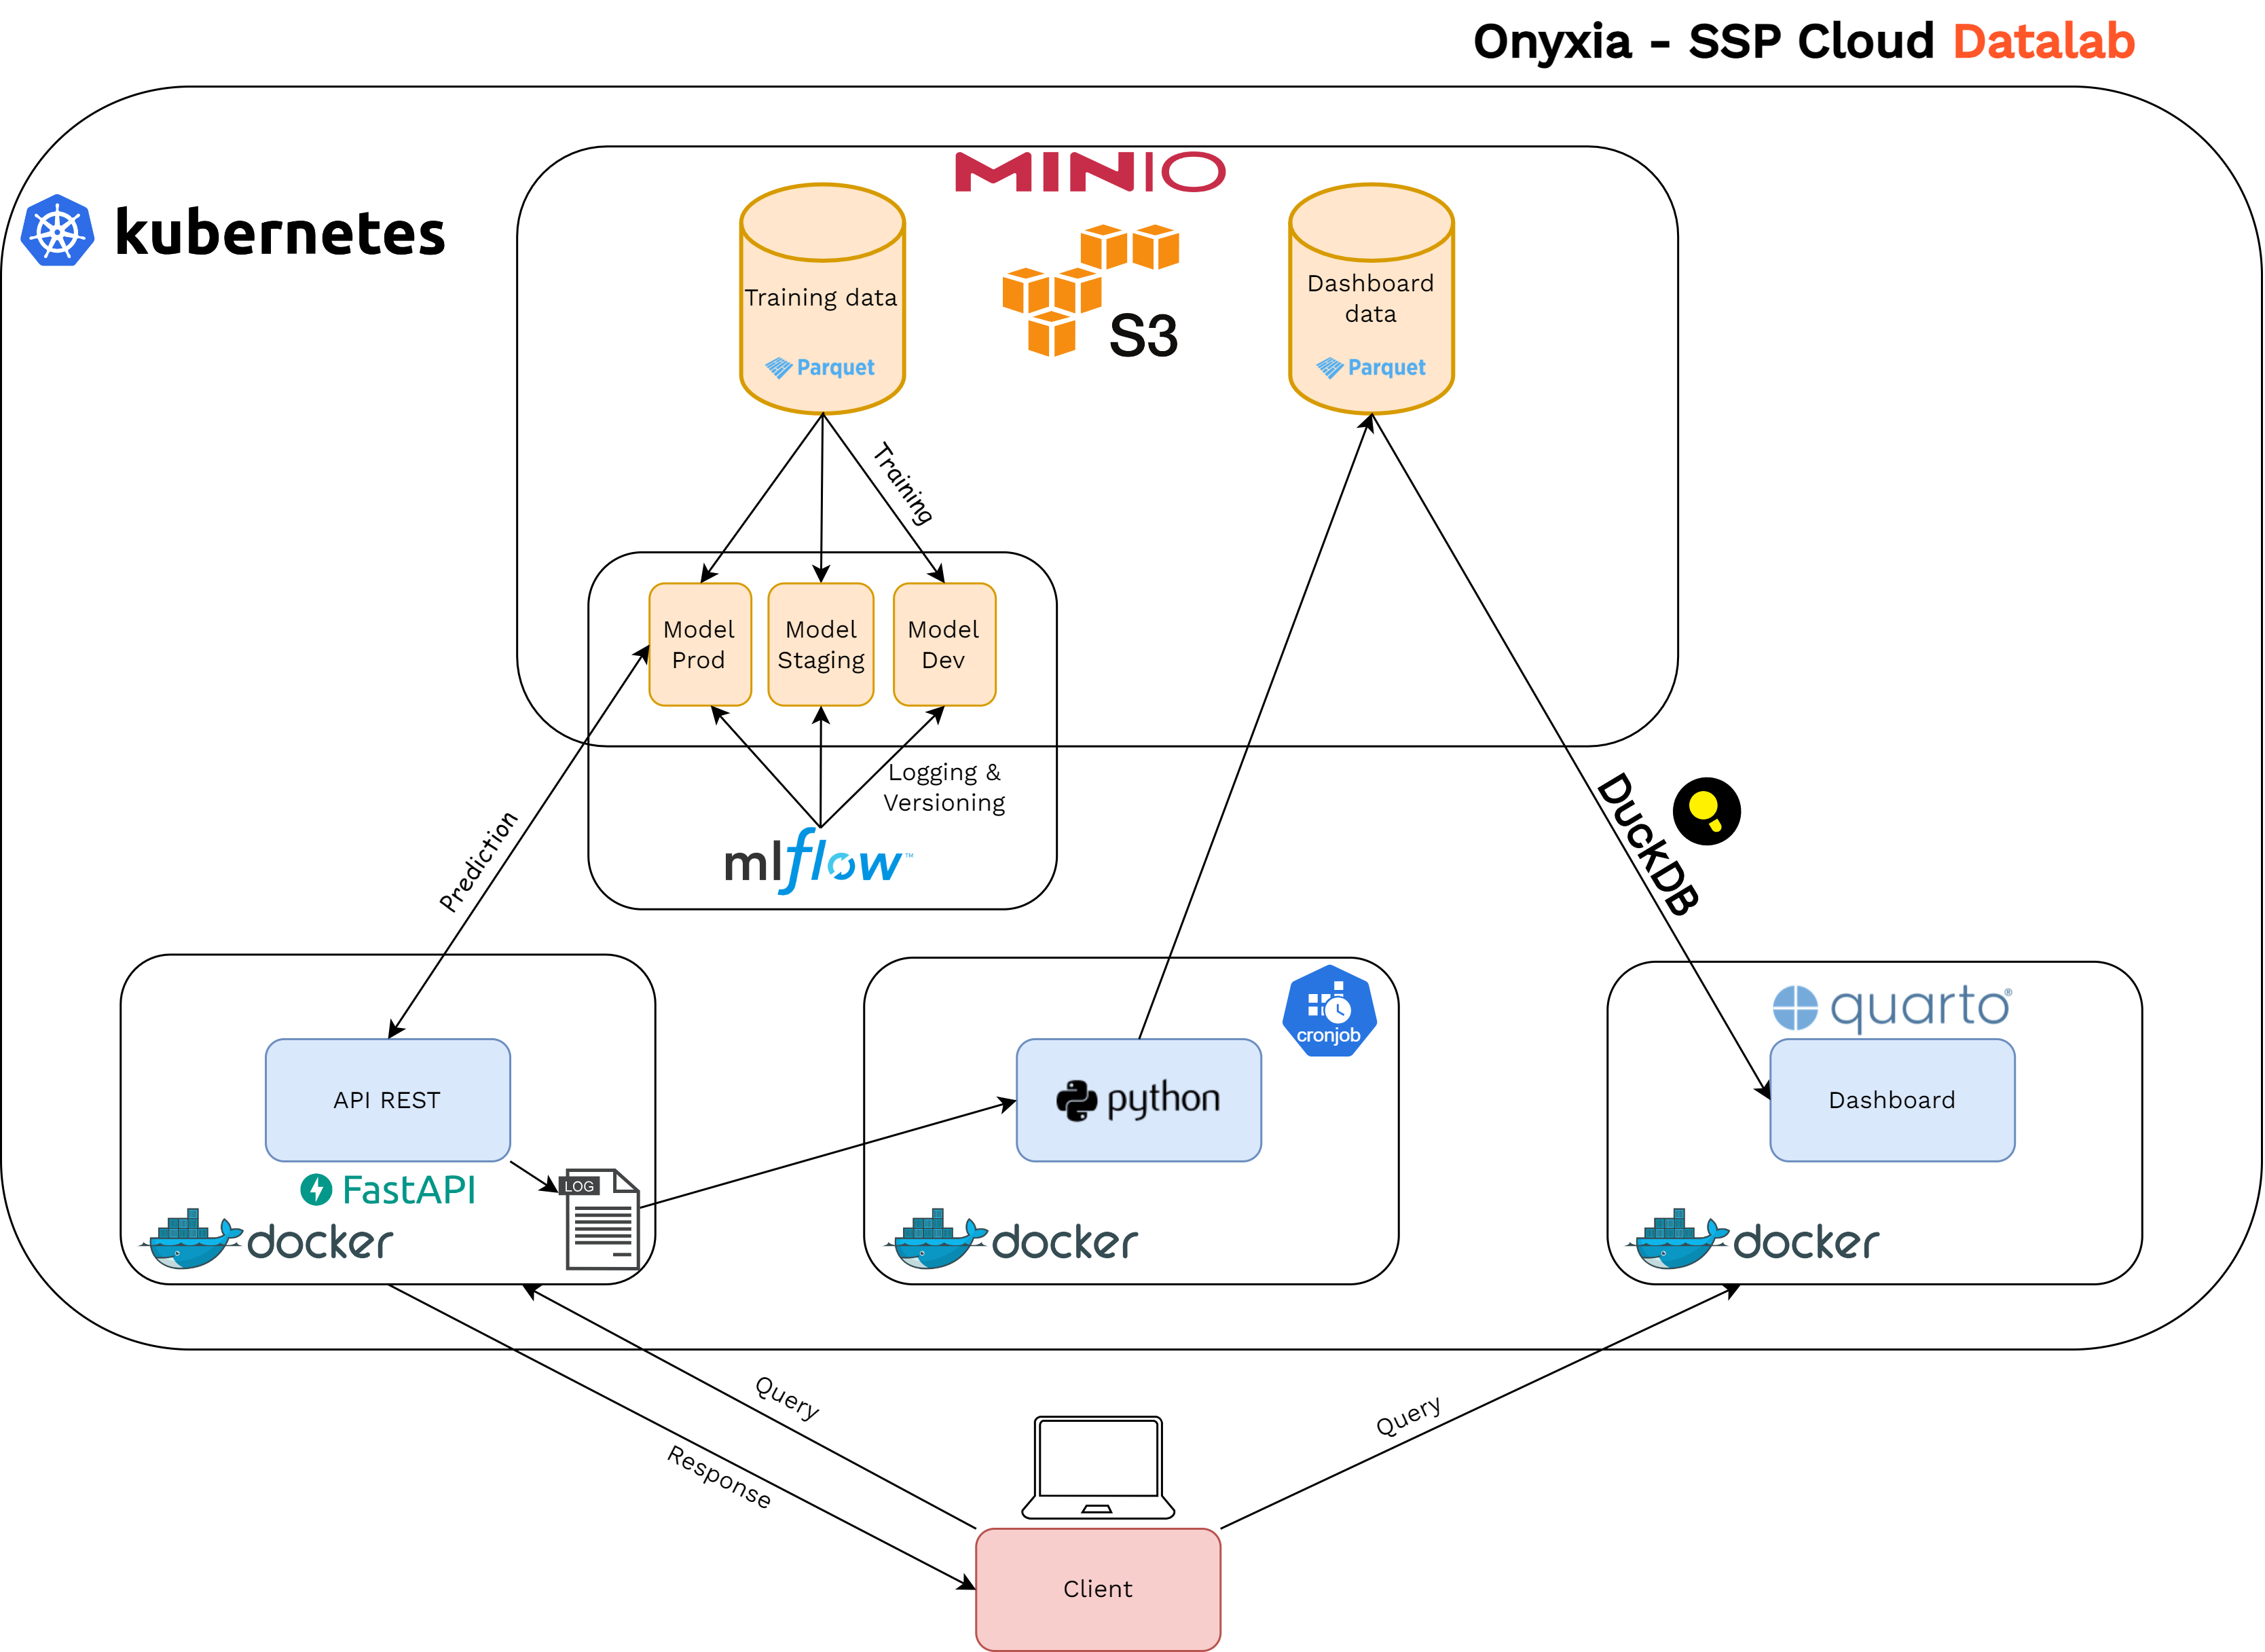
\includegraphics{../img/monitoring-datalab.pdf}
\end{center}

\subsection{Quality control}\label{quality-control}

\begin{itemize}
\tightlist
\item
  Test data is {\textbf{gathered and annotated periodically}}
\item
  Annotation is done with {\textbf{Label Studio}}
\item
  {\textbf{Performance metrics}} are computed on the test data
\item
  Performance is diplayed on the {\textbf{monitoring dashboard}}
\item
  {\textbf{Specific retraining}} is necessary when specific metrics
  decrease under a certain threshold (not done yet)
\end{itemize}

\subsection{Quality control}\label{quality-control-1}

\begin{center}
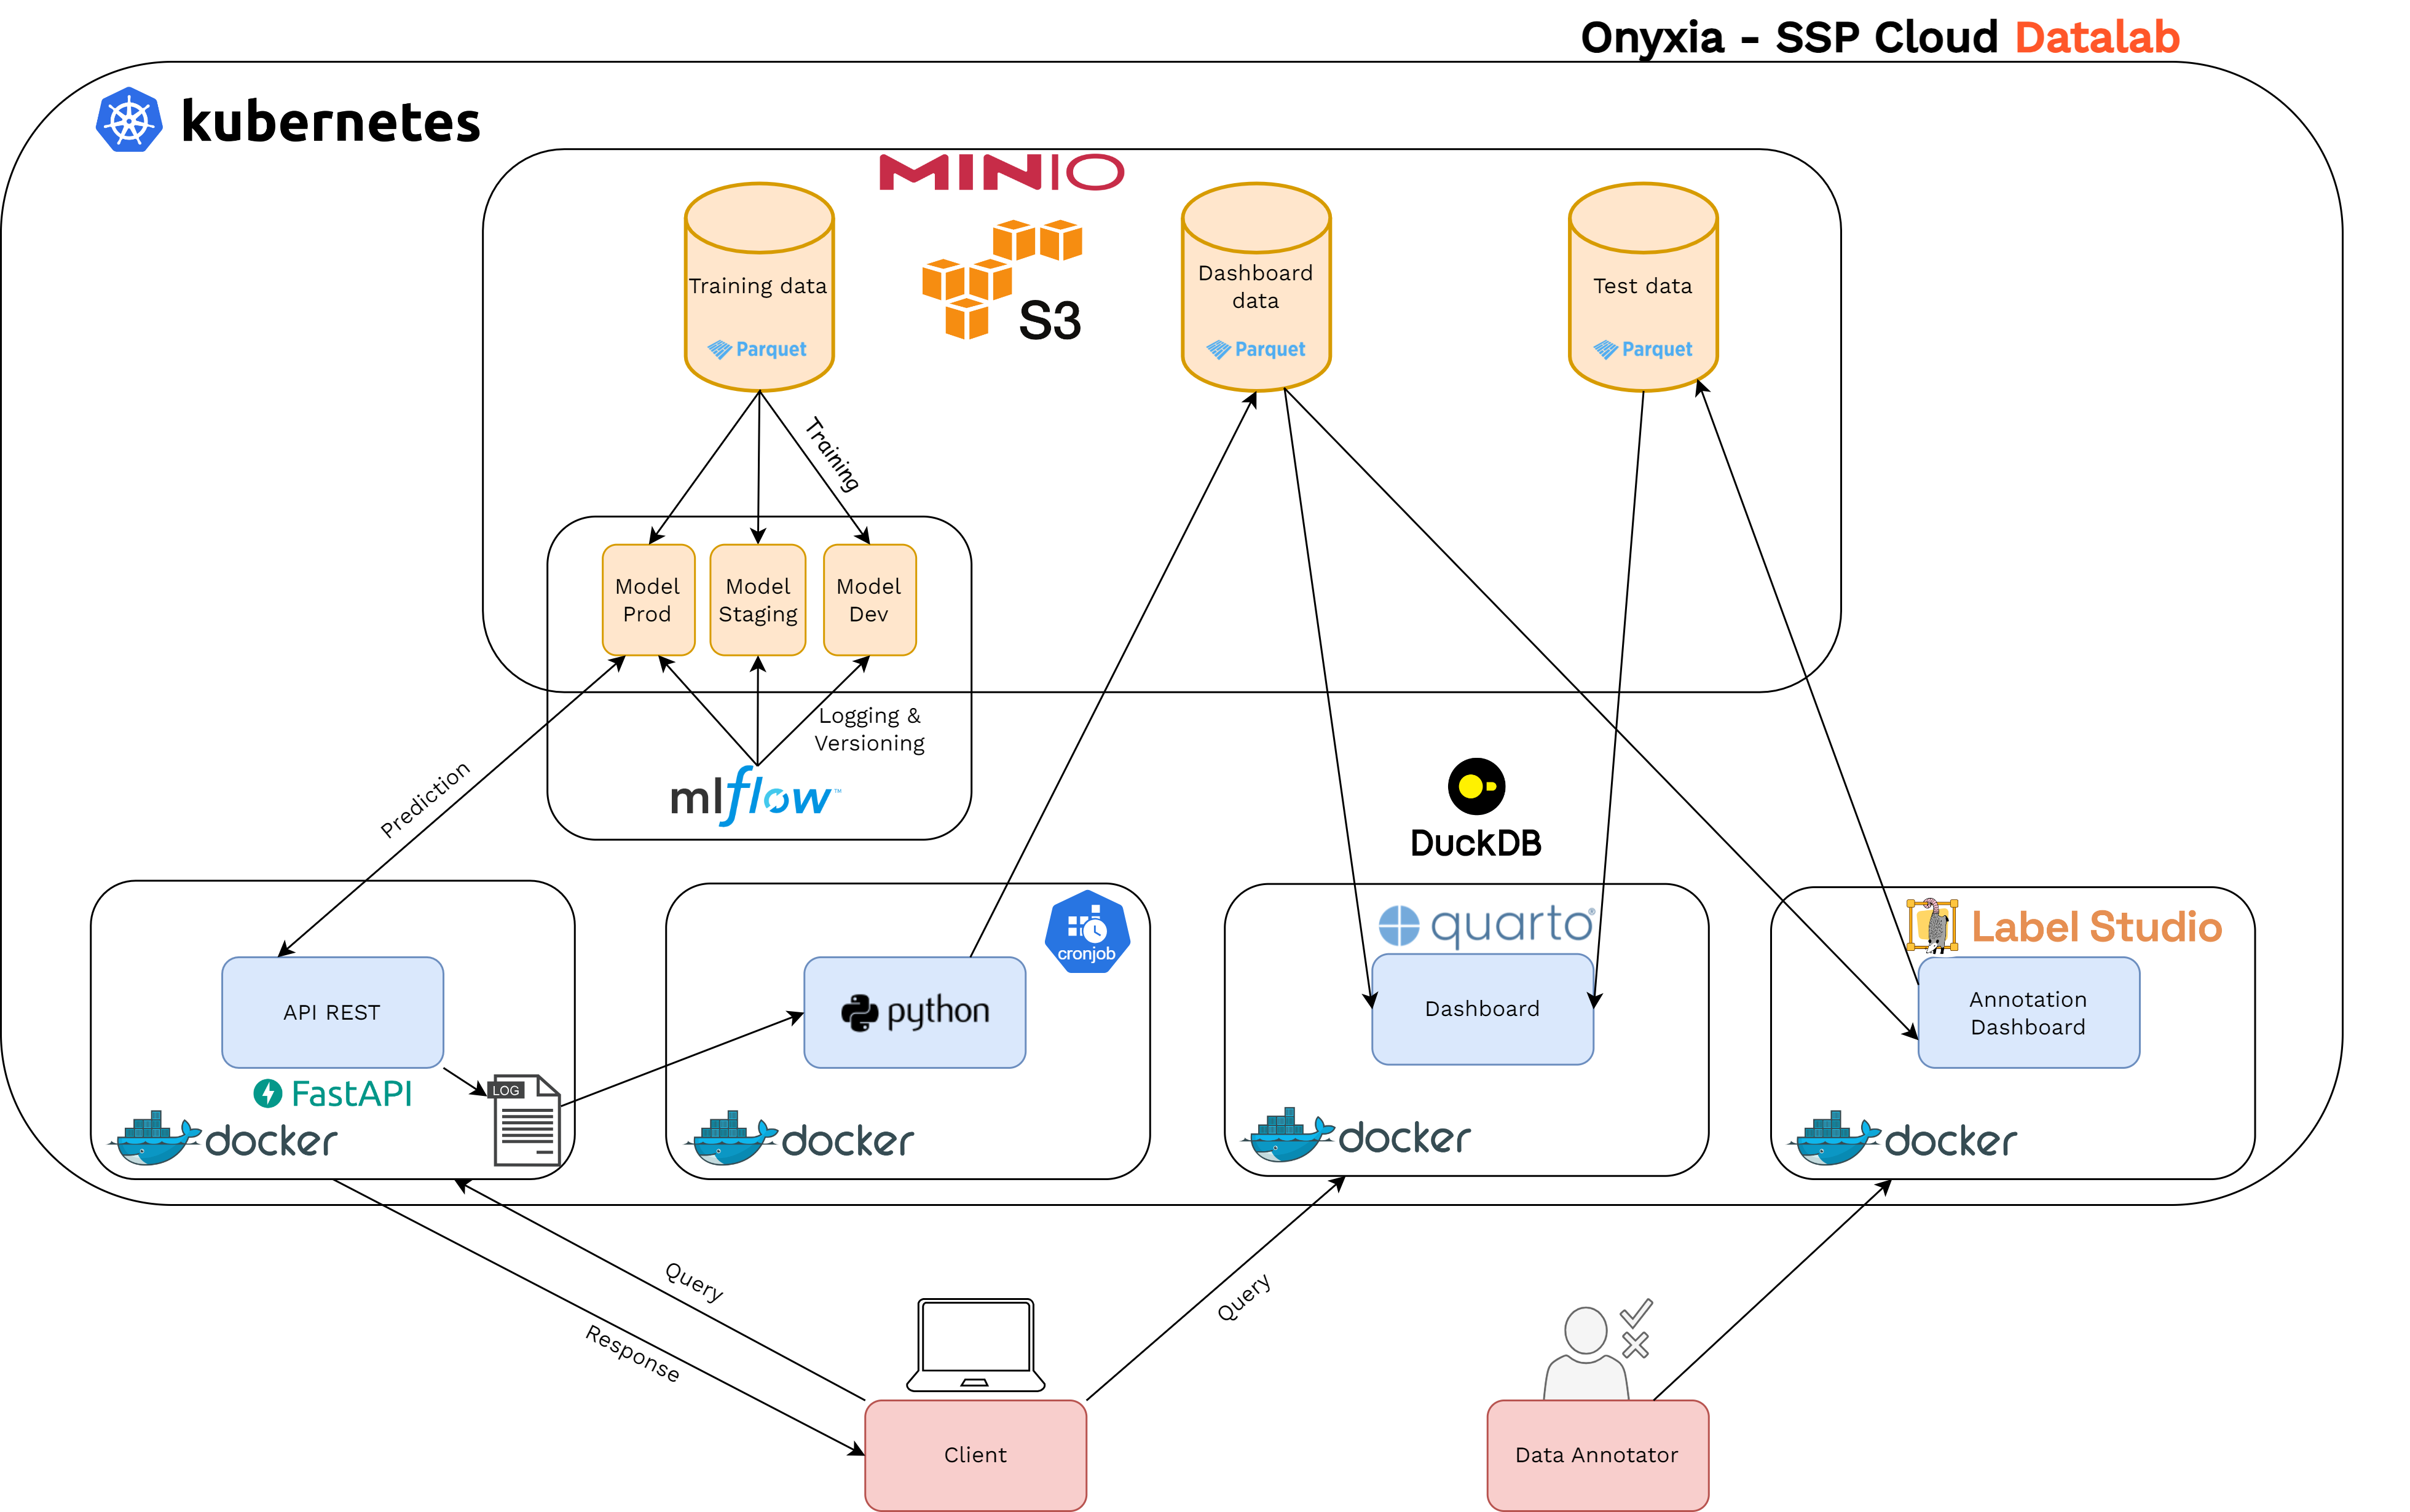
\includegraphics{../img/annotation-datalab.png}
\end{center}

\subsection{NACE revision : 1-to-1
correspondence}\label{nace-revision-1-to-1-correspondence}

\begin{itemize}
\tightlist
\item
  An easy and ideal case
\end{itemize}

\subsection{NACE revision : 1-to-many
correspondence}\label{nace-revision-1-to-many-correspondence}

\begin{itemize}
\tightlist
\item
  An ultimately less desirable solution
\item
  Need human decision on textual description
\end{itemize}

\subsection{Strategy for the flow of
formalities}\label{strategy-for-the-flow-of-formalities}

Business knowledge to specify the ``practical'' correspondence table: -
in practice, is it really a 1-to-many situation ? - In progress
{\textbf{Kubernetes cluster}} - Experiment tracking and model store:
{\textbf{MLflow}} - Model served via an API: {\textbf{FastAPI}} -
Automation with {\textbf{ArgoCD}} - Monitoring dashboard:
{\textbf{Quarto}} and {\textbf{DuckDB}} - Quality control: annotations
with {\textbf{Label Studio}}

\subsection{Strategy for the stock}\label{strategy-for-the-stock}

\begin{itemize}
\tightlist
\item
  {\textbf{Argo Workflows}} used for \emph{distributed} training
\item
  {\textbf{MLflow}} used to track/log experiments and compare runs
\item
  Custom model class allows to package {\textbf{pre-processing steps}}
  in the \texttt{predict} method:
\end{itemize}

\subsection{API serving}\label{api-serving-2}

\begin{itemize}
\tightlist
\item
  Text classification model served through a containerized {\textbf{REST
  API}}:

  \begin{itemize}
  \tightlist
  \item
    {\textbf{Simplicity}} for end users
  \item
    {\textbf{Standard query format}}
  \item
    {\textbf{Scalable}}
  \item
    {\textbf{Modular}} and {\textbf{portable}}
  \end{itemize}
\item
  {\textbf{Multiple endpoints}}: batch, online
\item
  Continuous deployment with {\textbf{Argo CD}}
\end{itemize}

\subsection{API serving}\label{api-serving-3}

\begin{center}
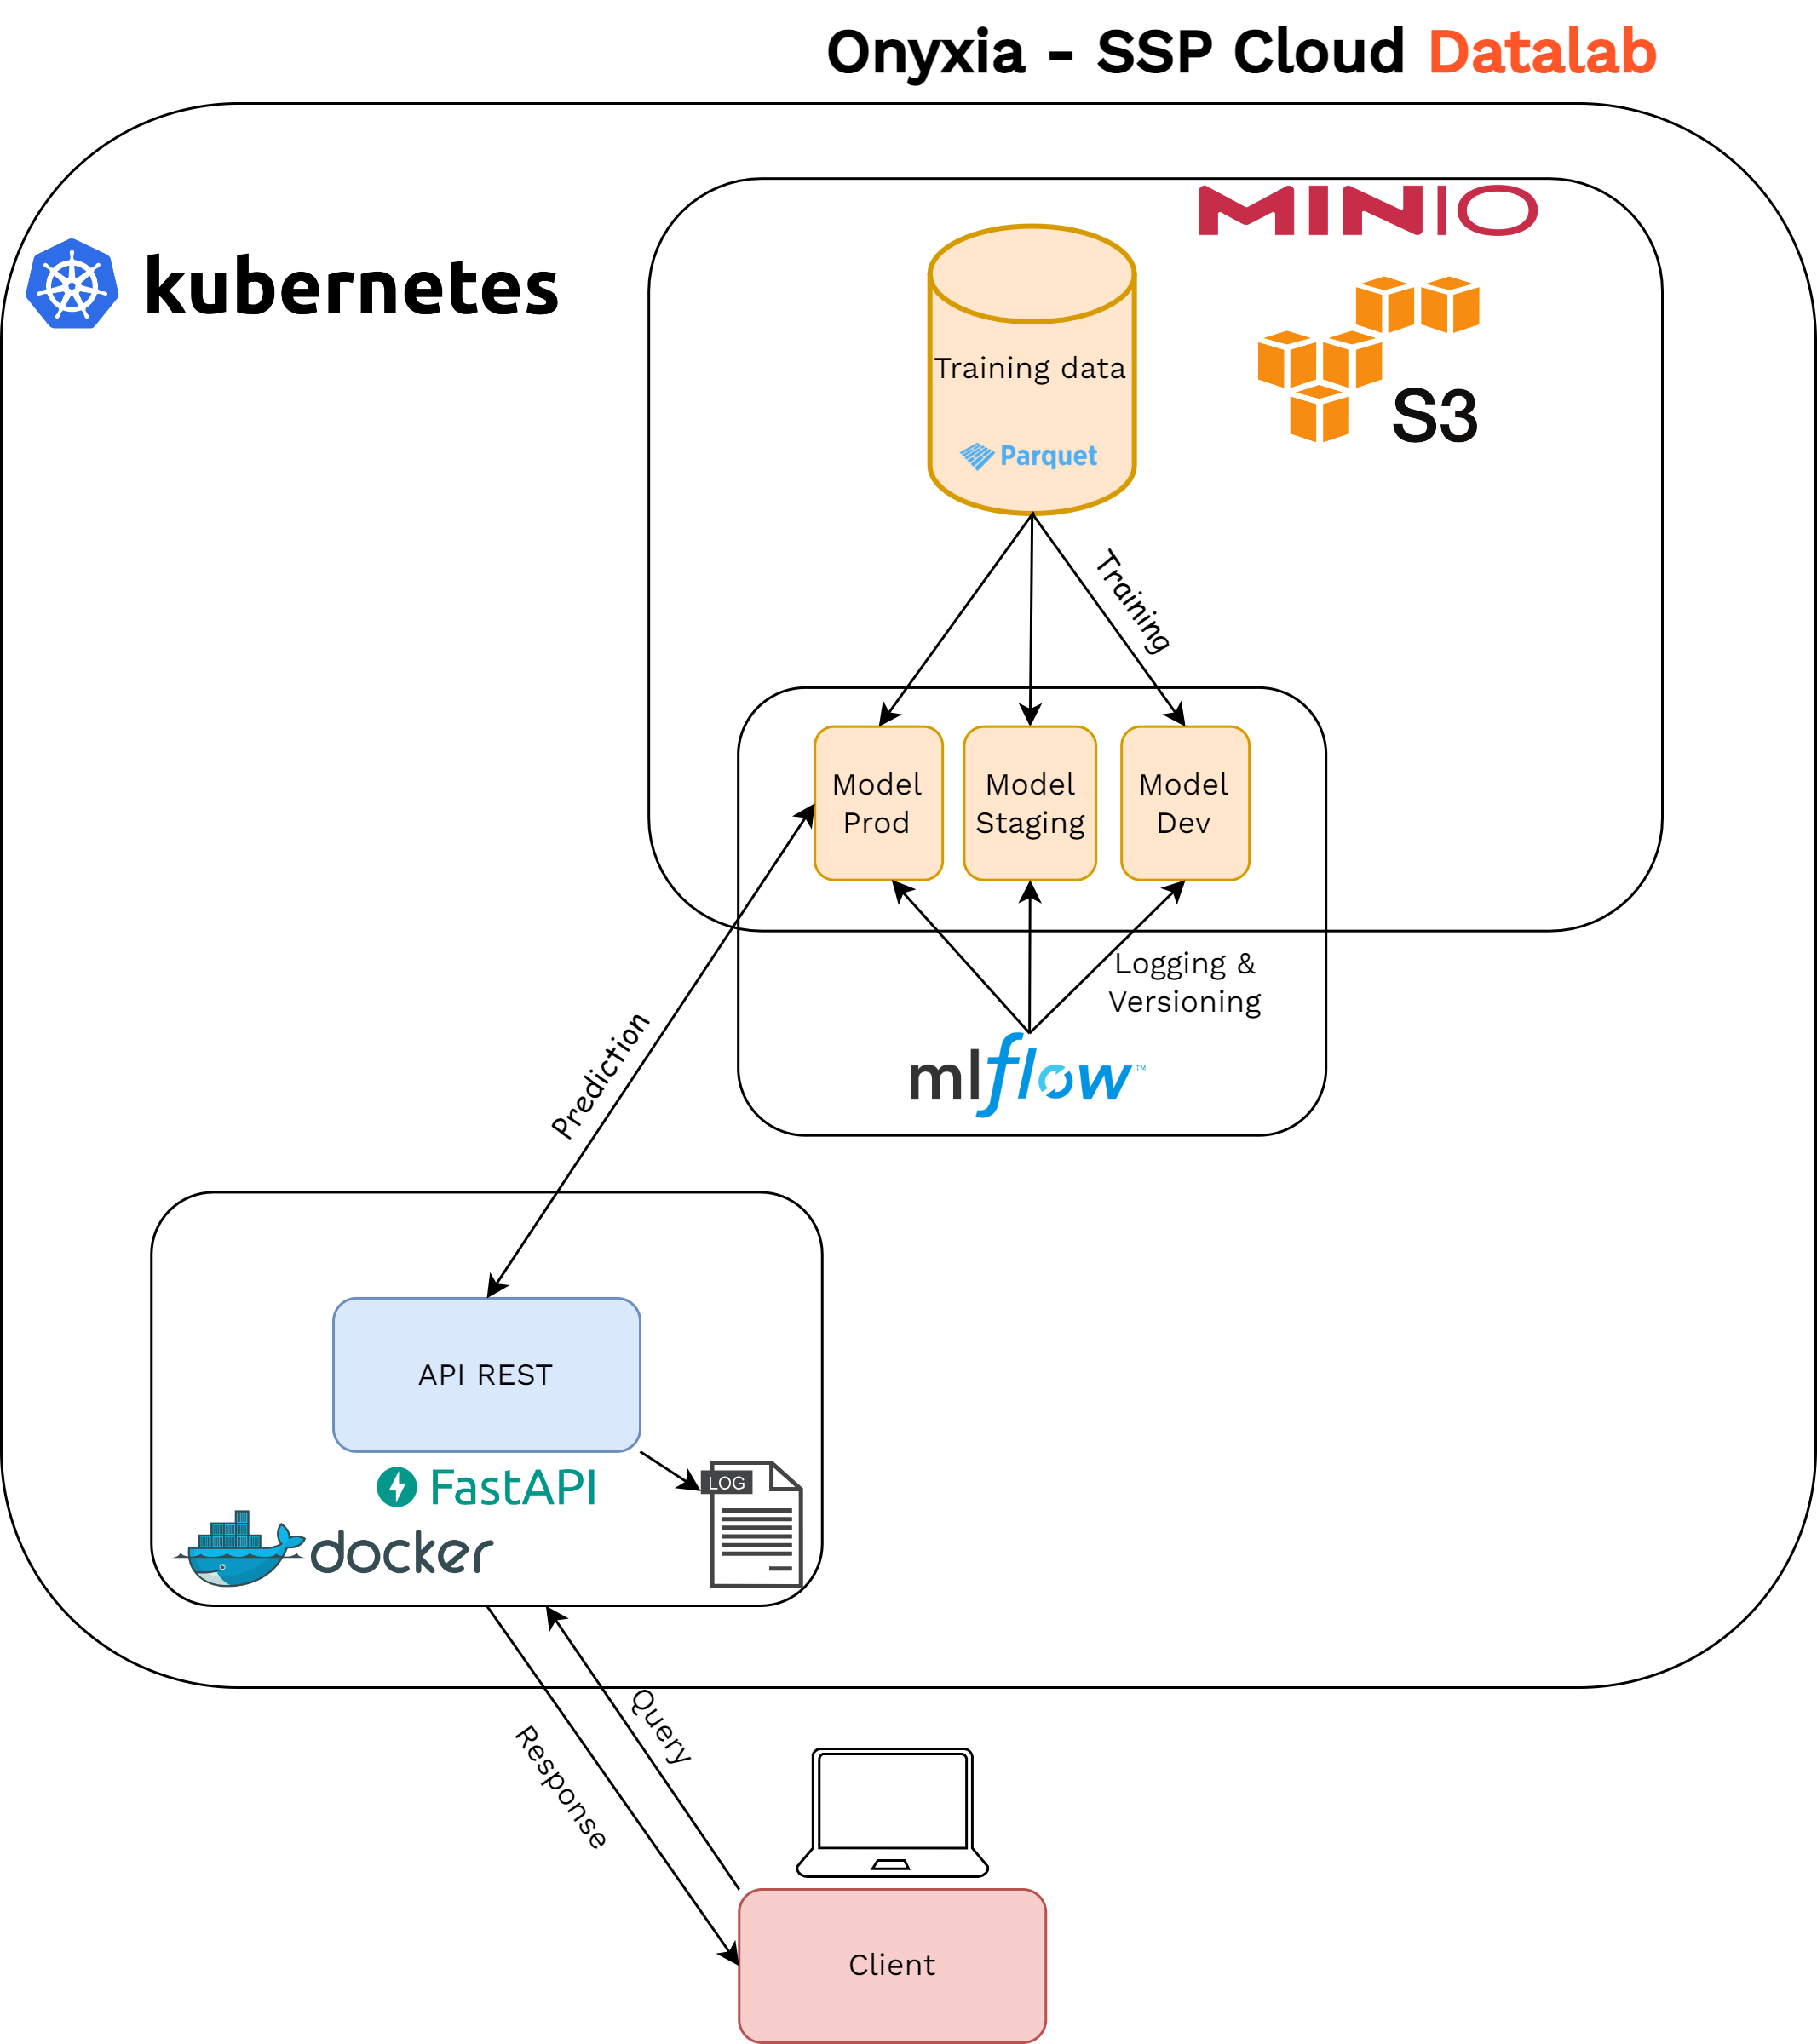
\includegraphics{../img/api-datalab.png}
\end{center}

\subsection{Monitoring}\label{monitoring-3}

\begin{itemize}
\tightlist
\item
  {\textbf{Monitoring}} the model in a production environment is
  necessary:

  \begin{itemize}
  \tightlist
  \item
    To detect {\textbf{distribution drifts}} in input data
  \item
    To check that the model has a {\textbf{stable behavior}}
  \item
    To decide {\textbf{when to retrain}} a model
  \end{itemize}
\item
  Ideally, we would like to track model {\textbf{accuracy in real-time}}
  but expensive
\item
  In addition, monitoring of the API: {\textbf{latency}},
  {\textbf{memory managment}}, {\textbf{disk usage}}, etc.
\end{itemize}

\subsection{Monitoring}\label{monitoring-4}

\begin{itemize}
\tightlist
\item
  {\textbf{How}} we do it:

  \begin{itemize}
  \tightlist
  \item
    API {\textbf{logs}} its activity
  \item
    Logs are fetched and formatted {\textbf{periodically}}
  \item
    {\textbf{Metrics}} are computed from the formatted logs
  \item
    Display on a {\textbf{dashboard}}
  \end{itemize}
\end{itemize}

\subsection{Monitoring}\label{monitoring-5}

\begin{center}
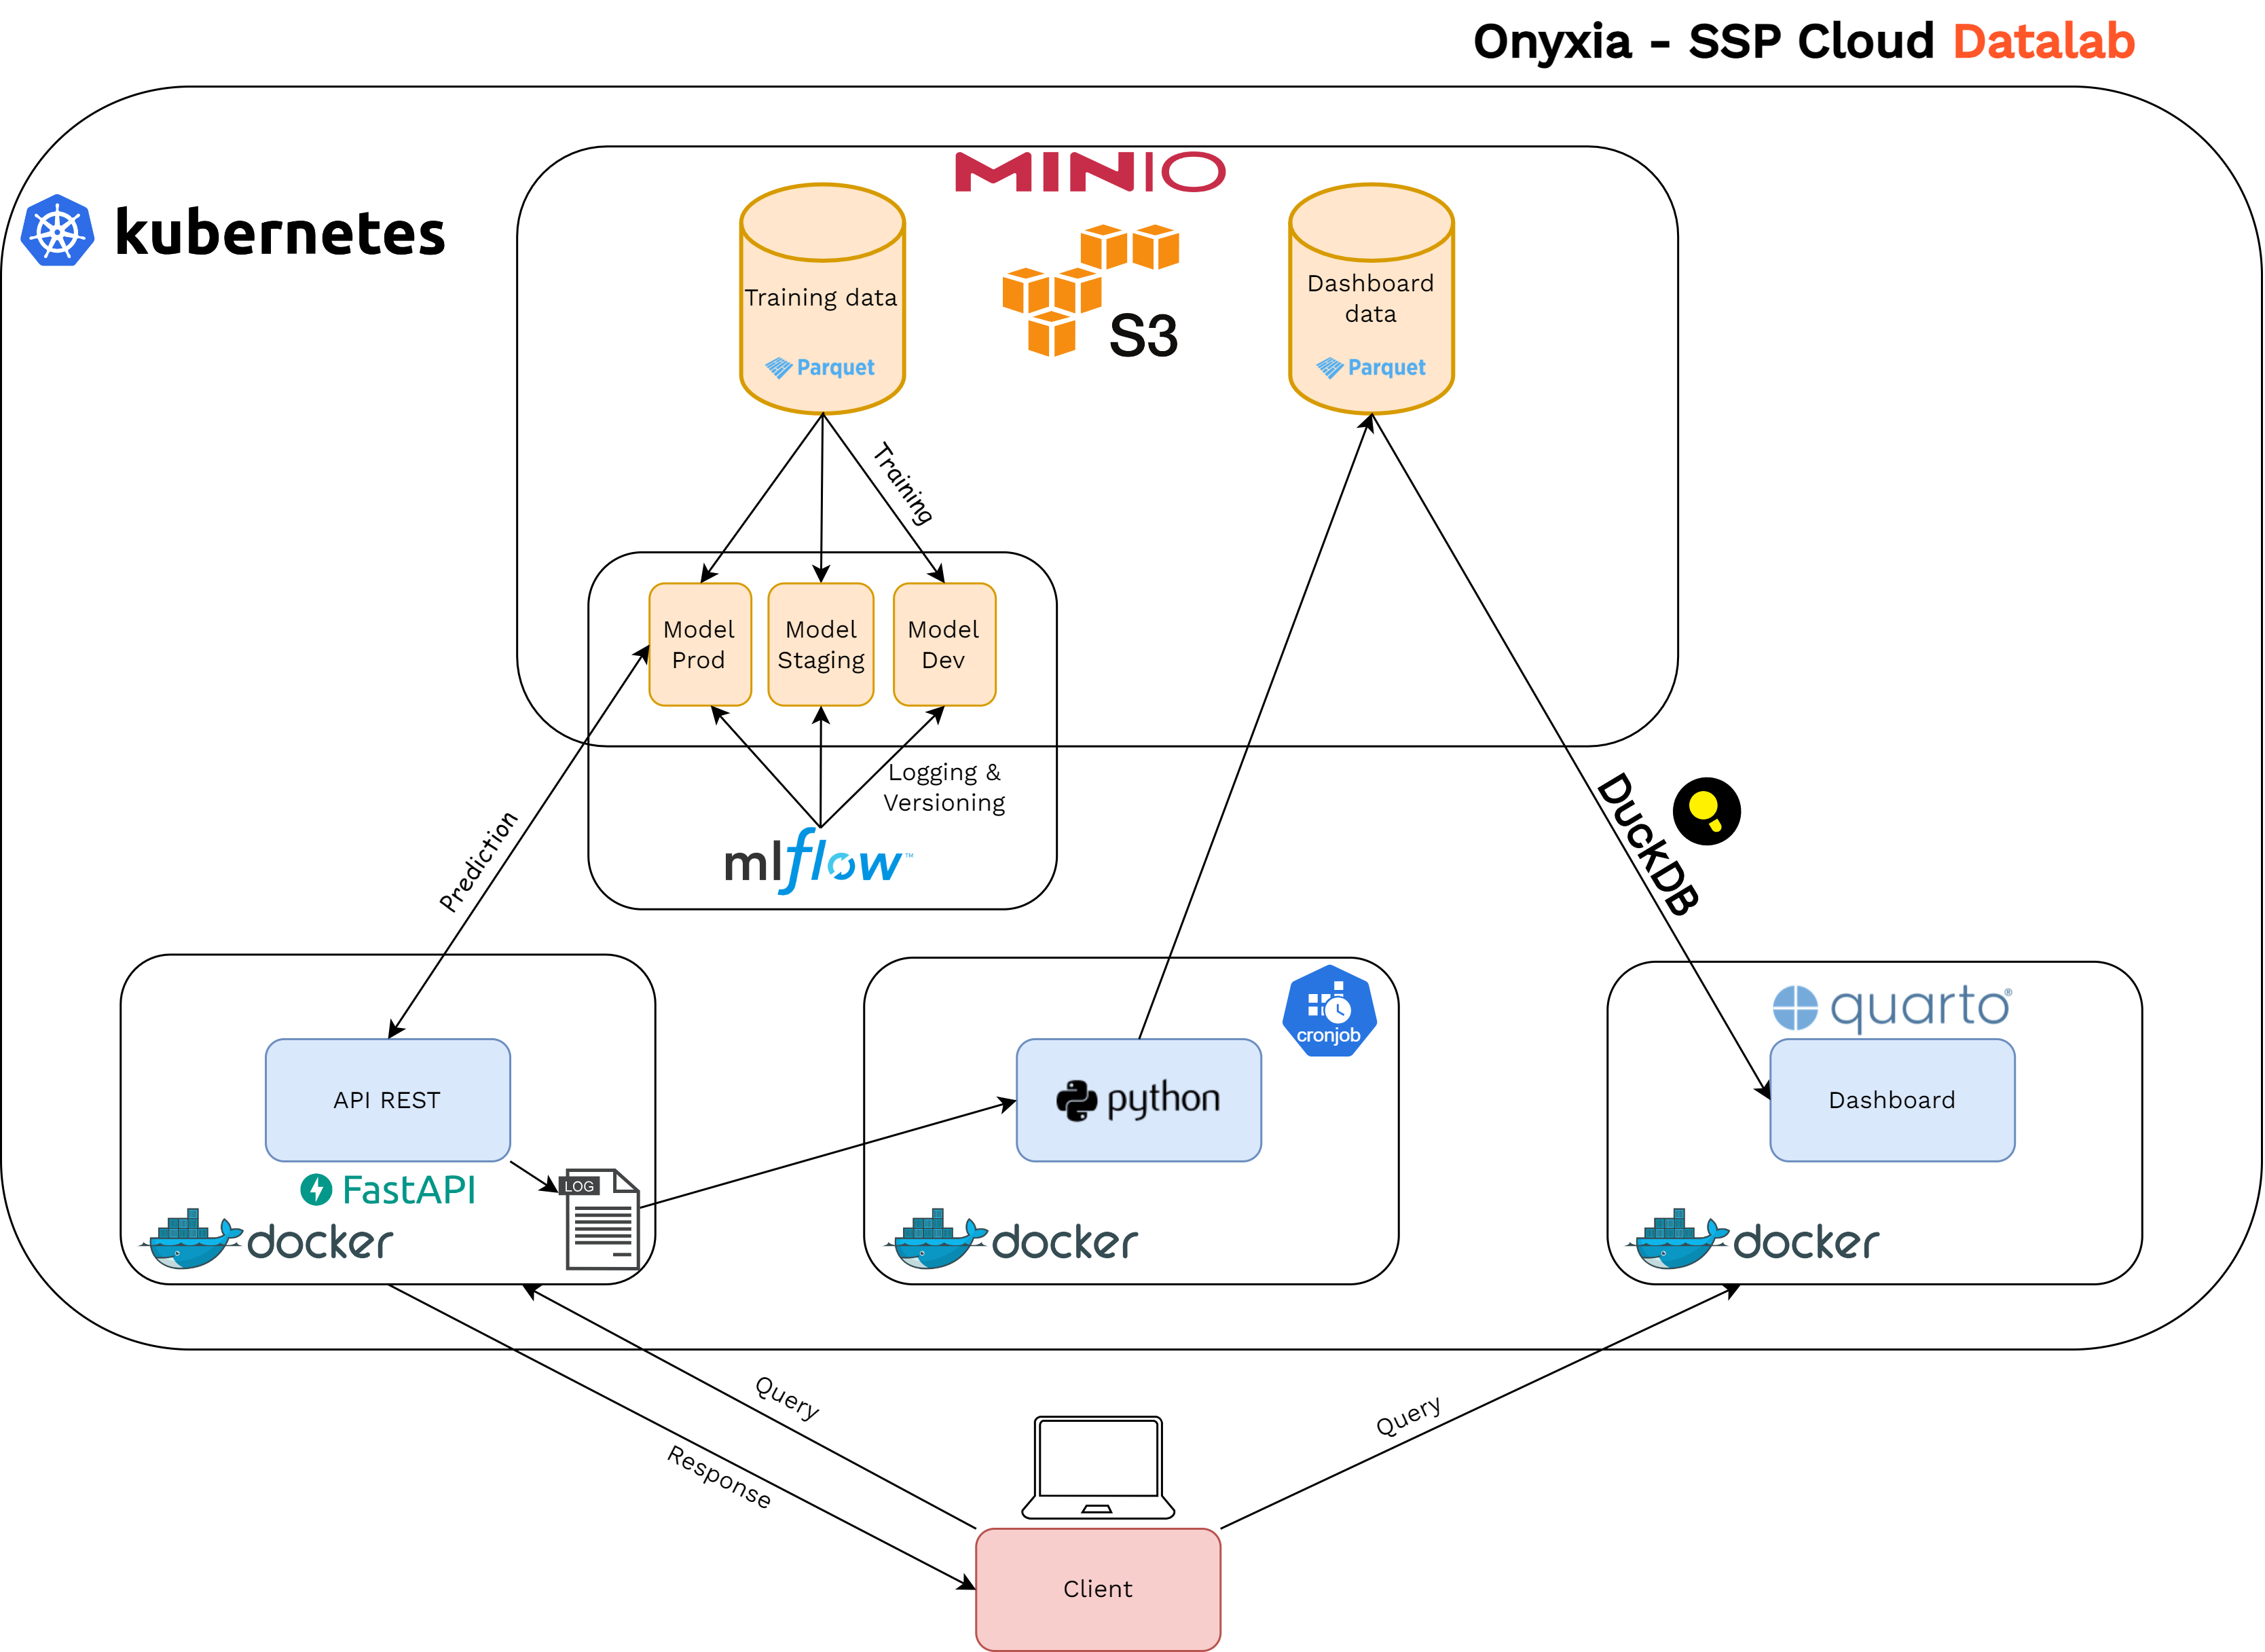
\includegraphics{../img/monitoring-datalab.pdf}
\end{center}

\subsection{Quality control}\label{quality-control-2}

\begin{itemize}
\tightlist
\item
  Test data is {\textbf{gathered and annotated periodically}}
\item
  Annotation is done with {\textbf{Label Studio}}
\item
  {\textbf{Performance metrics}} are computed on the test data
\item
  Performance is diplayed on the {\textbf{monitoring dashboard}}
\item
  {\textbf{Specific retraining}} is necessary when specific metrics
  decrease under a certain threshold (not done yet)
\end{itemize}

\subsection{Quality control}\label{quality-control-3}

\begin{center}
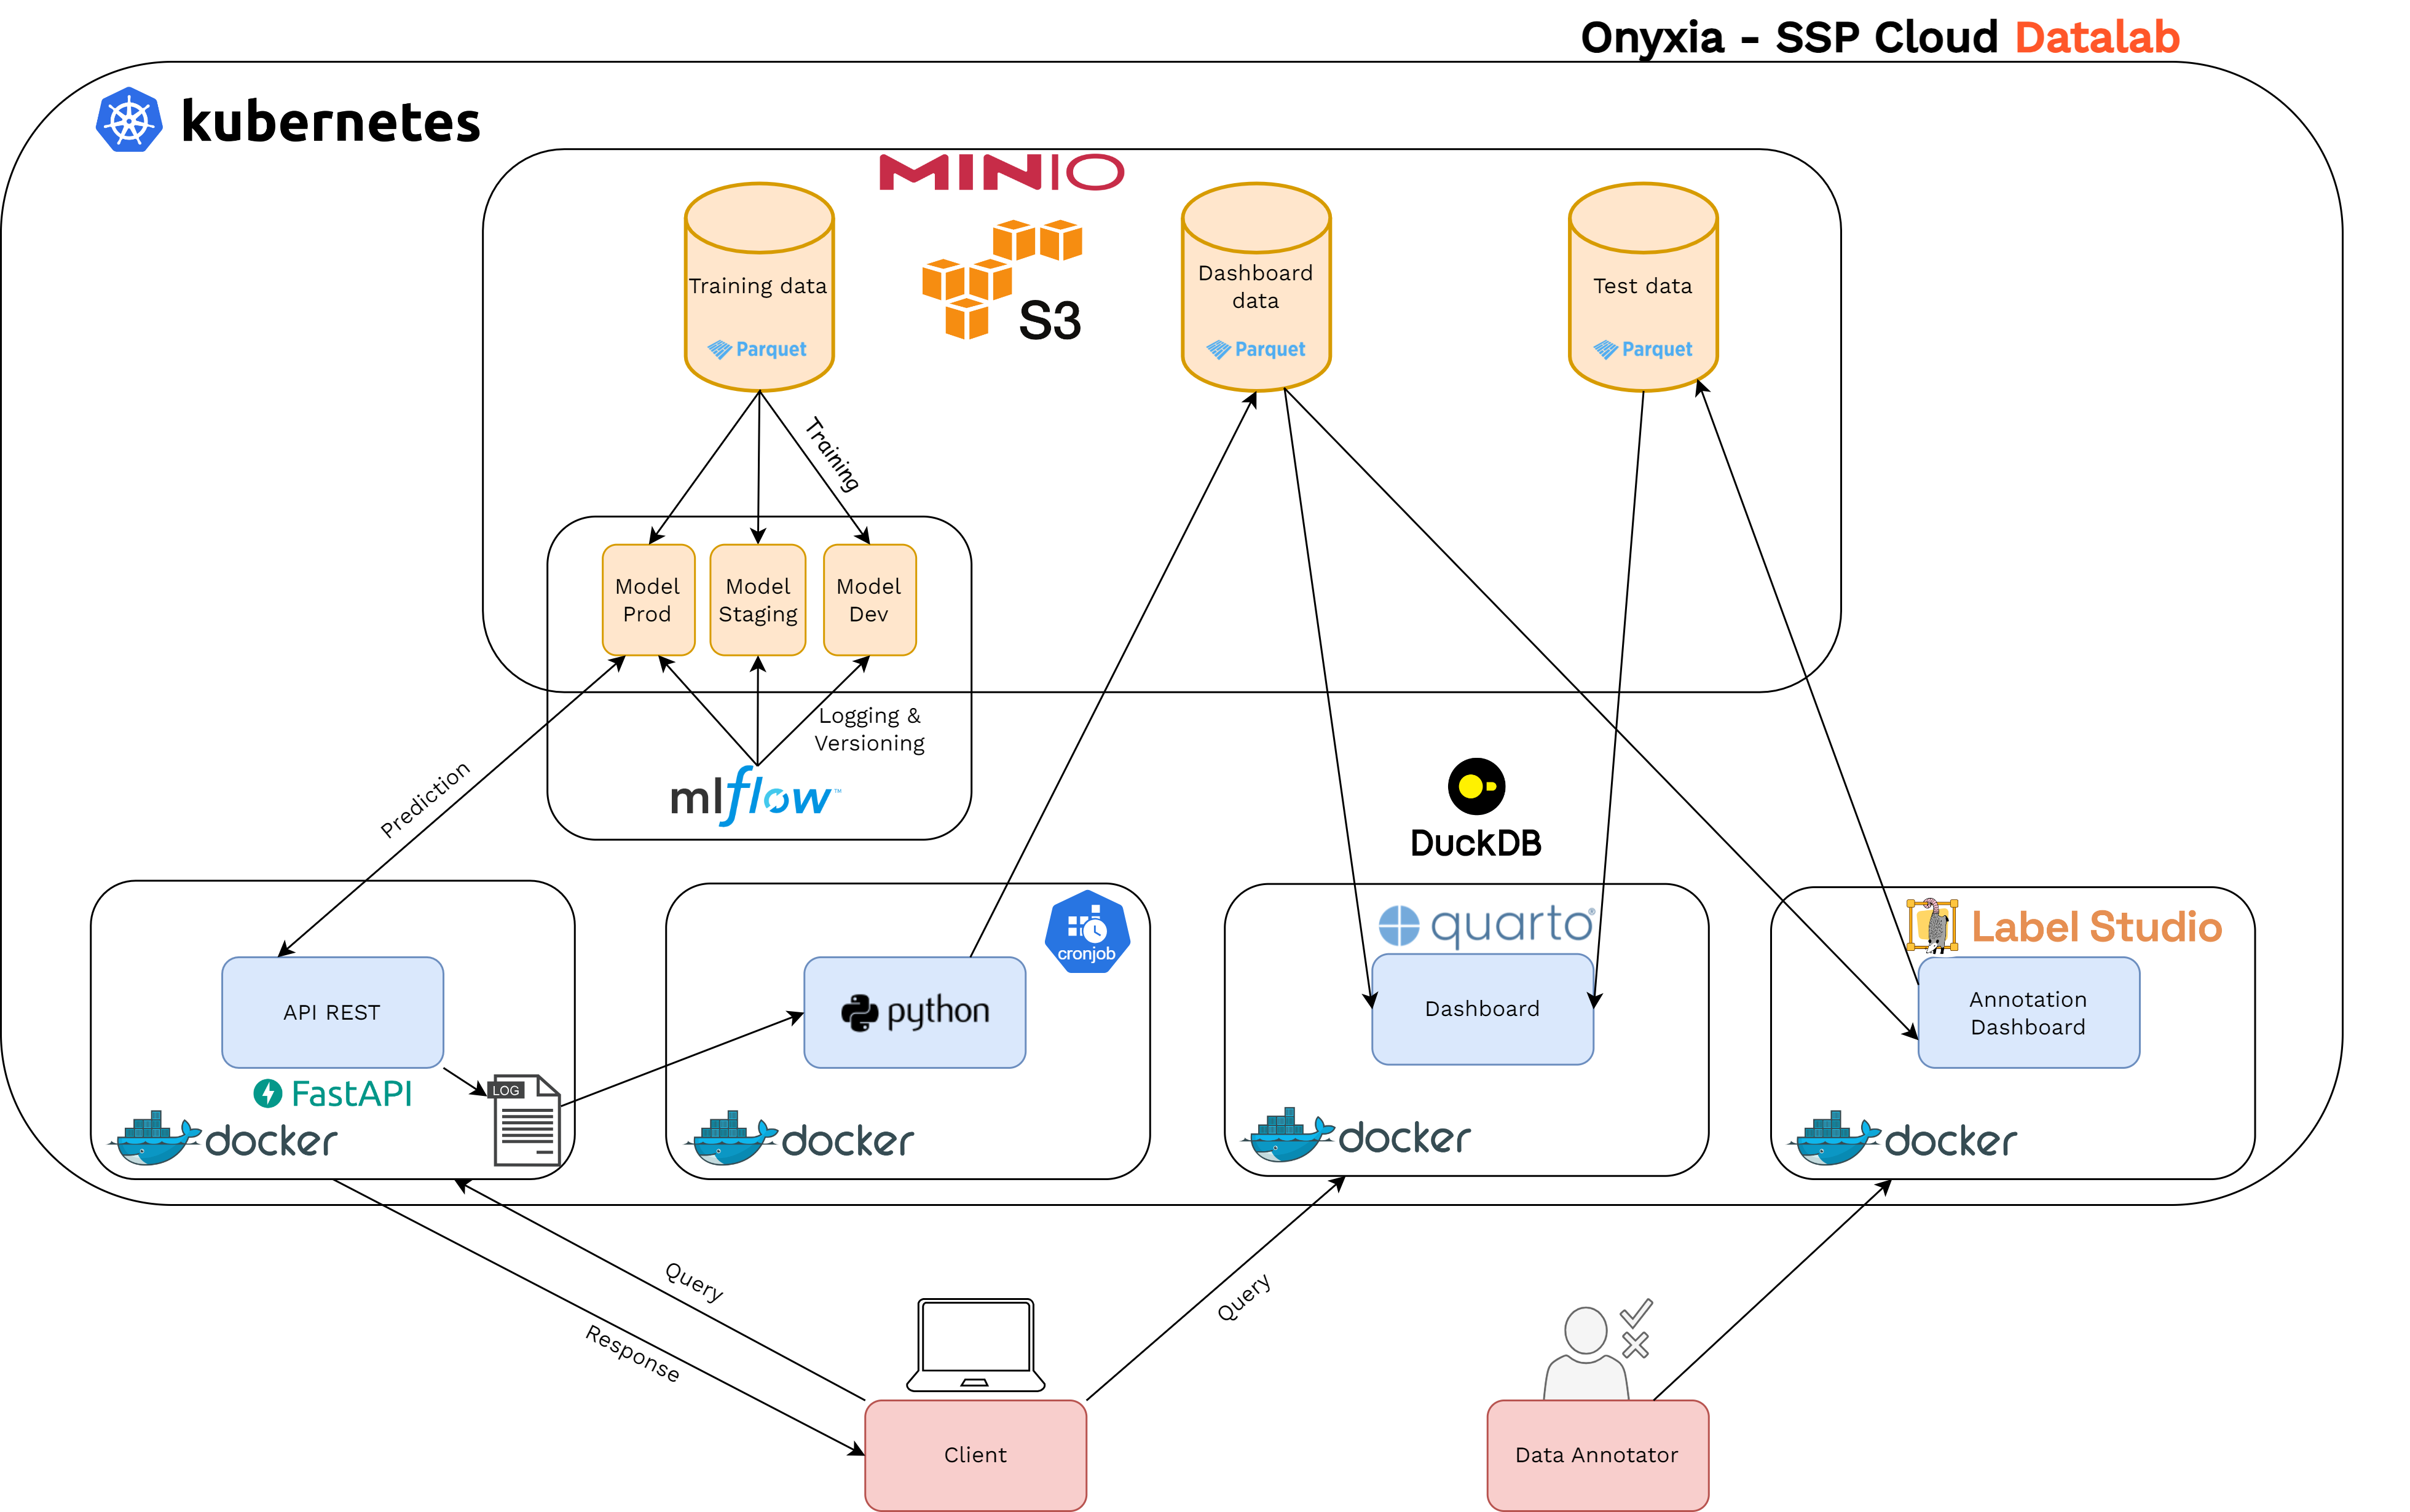
\includegraphics{../img/annotation-datalab.png}
\end{center}



\end{document}
